\chapter{Wstęp}

\section{Ataki rekonesansowe}
Ataki rekonesansowe są typem ataków komputerowych których głównym celem jest pozyskanie informacji na temat atakowanego systemu bądź podatności które w nim występują. Słowo ,,rekonesans'' zostało zapożyczone z militarnej nomenklatury oknoszące się do zapoznania z terenem wroga. W kontekście ataków na sieci komputerowe stwierdzeniem określa się analogiczny krok -- działanie przed właściwym atakiem. Sam rekonesans można podzielić dodatkowo na dwie kategorie:
\begin{enumerate}
	\item aktywny atak rekonesansowy,
	\item pasywny atak rekonesansowy.
\end{enumerate}
Atak aktywny odnosi się do działania, gdy atakujący podejmuje akcje przez które może wchodzić w interakcję z systemem, na przykład wysyłanie specjalnie spreparowanych zapytań czy skanowanie portów.

Atak pasywny to tylko i wyłącznie obserwacje działającego systemu. Może to być na przykład podsłuchiwanie ruchu, analiza najczęściej odwiedzanych stron, czy choćby przyglądanie się innym procesom aby opowiednio przyrgotować atak właściwy.

Obie wersje ataków rekonesansowych są również częścią tak zwanego etycznego hakowania (ang. \textit{ethical hacking}). Osoby które tym się zajmują (określani po angielsku jako \textit{white hat}) starają się wytknąć błędy i podatności w systemach przy czym starają się nie ingerować w ich działanie.

Rekonesans DNS jest częścią testu penetracyjnego polegającą na pozyskaniu jak największej ilości informacji na temat badanej domeny. Dane uzyskiwane podczas niego odnoszą się zarówno do serwera DNS jak i wpisów które on przechowuje. Zebrane informacje mogą kompromitować infrastrukturę sieciową firmy nie powodując przy tym generowania zbyt podejrzanego ruchu. Między innymi dlatego ważne jest, aby przywiązywać znaczną uwagę do tego kto i w jaki sposób próbuje łączyć się z serwerami autorytatywnymi odpowiedzialnymi za domenę.


AXFR (\textit{ang. Asynchronous Xfer Full Range}) to mechnizm używany w protokole DNS (\textit{Domain Name System}) do transferowania strefy za którą odpowiada serwer nazw. Głównym przeznaczeniem opisywanego standardu był transfer informacji pomiedzy podstawowym i zapasowanym serwerem przestrzeni nazw. Zasada jego działania jest bardzo prosta -- serwer podrzędny (\textit{ang. slave}) przesyła rządanie AXFR do serwera podstawowego (\textit{ang. primary, master}).

Oczywiste jest, że AXFR został wykorzystywany w celach zupełnie innych niż te, do których go zaprojektowano. Mowa tu o sytuacji, w której serwer główny w żaden sposób nie weryfikuje po swojej stronie źródła takiego zapytania. Prowadzi to do sytuacji, w której każdy, kto jest w stanie utworzyć odpowiedni pakiet TCP może wejść w posiadanie informacji o całej strefie, za którą odpowiada odpytywany serwer DNS. Wspomniane przygotowanie pakietu DNS nie jest specjalnie trudne, ponieważ umożliwia to wiele narzędzi, na przykład dig, wchodzący w skład pakietu bind. 

\section{Domain Name System}
Głównym zadaniem protokołu DNS (\textit{Domain Name System}) jest translacja nazw przyswajalnych dla użytkowników (najczęściej alfanumerycznych) na nazwy sieciowe, czyli adresy IP. 

System DNS ma charakterystyczną, hierarchiczną strukturę, którą zaprezentowano na rysunku \ref{hierarchy_dns}. Na rysunku przedstawiono węzeł główny (ang. \textit{root}) reprezentowany jako znak pojedyńczej kropki oraz przykład dwóch typów domen pierwszego poziomu.

\begin{center}
	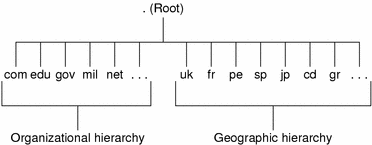
\includegraphics[scale=1]{image/hierarchy_dns}\label{hierarchy_dns}
\end{center}

Jeśli chodzi o podział domen pierwszego poziomu ze względu na przynależność organizacyjną, to aktualny stan przedstawiony jest w tabeli poniżej.

\begin{table}[]
	\centering
	\caption{Podział domen najwyższego poziomu ze względu na działalność.}
	\label{my-label}
	\begin{tabular}{ll}
		\hline
		com & Jednostki o działalności komercyjnej (ang. \textit{commercial institutions}) \\
		\hline
		edu & Jednostki edukacyjne (ang. \textit{educational institutions})\\
		\hline
		gov & Instytucje rządowe (ang. \textit{government institutions}) \\
		\hline
		mil & Grupy wojskowe (ang. \textit{military groupos}) \\
		\hline
		net & grupy związane z działaniem sieci (ang. \textit{network support centers}) \\
		\hline
		org & Organizacje nonprofit i inne (ang. \textit{nonprofit organizations}) \\
		\hline
		int & Organizacje międzynarodowe (ang. \textit{international organizations}) \\
		\hline 
	\end{tabular}
\end{table}

Przedstawiony podział nie jest stały. Autorzy zastrzegli, że w przysłości może być on rozszerzony o dodatkowe kategorie.

Podział ze względu na położenie geograficzne jest oczywiście bardziej naturalny i łatwy zarówno do wdrożenia jak i zrozumienia. Każdemu z państw przydzielono dwu bądź trzyliterowy identyfikator, który reprezentują domenę najwyższego poziomu odpowiadającą danemu państwu. Powołując się na informacje przedstawione na grafice \ref{hierarchy_dns} TLD o identyfikatorze \textit{uk} odpowiada domenom utożnasmianym z Wielką Brytnią, a \textit{fr} -- domenom francuskim.

Hierarchia systemu DNS wynika z faktu, że domenami internetowymi każdego poziomu może zarządzać inna organizacja. Odnosi się to zarówno do domeny \textit{root}, jak i domen nawyższego poziomu niezależnie od przynależności grupowej. W Polsce identyfikatorem TLD jest sufiks \textit{pl}, a jednostką odpowiedzialną za nią jest CERT Polska \cite{cert}. Jeśli użytkownik chciałby dołączyć ze swoją siecią do internetu powinien zgłosić do odpowiedniej organizacji taką chęć oraz dostarczyć wszystkich niezbędnych informacji które są wymagane przez zarządcę. 

Bardzo ważnym punktem jest wspomniana w poprzednim akapicie ,,chęć'' dołączenia do internetu. Jeśli uzytkownik czy organizacja chcą używać protokołu DNS jedynie do użytku wewnętrznego, to nie ma rystrykcyjnych ograniczeń co do używanych nazw. Jeśli natomiast oczekuje się wystawienia domen w taki sposób, aby były widoczne z zewnątrz, to należy odpowiednio:
\begin{enumerate}
	\item zarejestrować nazwę domeny,
	\item pozyskać adres IP.
\end{enumerate}


\chapter{Przegląd dostępnych narzędzi}
Społeczność internetu oferuje bardzo szeroką gamę narzędzi umożliwiających pozyskiwanie informacji na podstawie protokołu DNS. Bardzo użytecznym i przydatnym narzędziem jest w tym przypadku program dig. Wspomniany program ma jednak znaczącą wadę -- jest wydajny jedynie przy niewielkiej liczbie odpytywanych domen. Dodatkową niedogodnością jest, wbrew pozorom, fakt, że program wchodzi w skład pakietu Open Source bind. Ten, jak każde oprogramowanie na wolnej licencji, cierpi na szereg niedogodności z tym związanych. Najbardziej prozaicznym problemem jest fakt, że oprogramowanie jest tworzone przez wiele osób, więc bardzo trudno zastosować jeden standard kodowania, gdyż każda z osób ma swój preferowany. Poza tym, dużą wadą jest trudność wprowadzania zmian w tego typu oprogramowaniu, wynikająca zarówno z punktu poprzedniego jak i ze złożoności programu, którą cechuje się dig w tym momencie.

Istnieją także inne pakiety implementujące w dość wydajny sposób klienta systemu DNS jak np. pjlib \cite{pjlib}. Również w tym przypadku można borykać się z problemami wynikającymi z założeń przyjętych przez twórców tego oprogramowania. Koknkretyzując to stwierdzenie - wspomniana biblioteka z założenia miała być wykorzystywana do protokołu SIP, a więc implementacja klienta DNS weszła w jej skład tylko i wyłączenie dlatego, że twórcy jej potrzebowali do innych celów. Implikuje to fakt, że pobieranie wiadomości jest niekompletne na płaszczyźnie typów wiadomości. Jednym z nich jest typ nr 252, czyli AXFR, który jest jednym z kluczowych elementów rekonsesansu na podstawie protokołu DNS.